% Additive, optional manuscript module. No existing project file is modified.
% Requires graphicx. All paths are relative to the Overleaf project root.
\section{MetaDrive: responsive traffic and a null primary method comparison}
\label{add20260923:metadrive:section}

\paragraph{Setting and scope.}
We evaluated six prespecified IDM-controller updates in a native MetaDrive
$4\!\rightarrow\!1\!\rightarrow\!4$-lane bottleneck with eight vehicles.
The focal vehicle is evaluated against seven background vehicles.
The proxy fixes the background controller parameters, while deployment selects
a shared background-controller profile separately for each candidate and for
the incumbent, maximizing the background vehicles' own mean return.
The short and long response conditions search 4 and 12 prespecified profiles
using two training scenarios per profile; this is finite controller search,
not neural-policy training or an exact best response.
The focal update is scored against the incumbent under their respective
induced responses. Native cumulative return is the outcome, and greater return
alone must not be interpreted as greater driving safety.
This is a custom response extension of MetaDrive, distinct from HighwayEnv
and from an official adaptive MetaDrive benchmark score.

\paragraph{Protocol and information boundary.}
The first cohort comprises four pilot roots, 12 calibration roots, and
30 independent confirmation roots. All six candidates are retained, including
proxy-negative candidates. Response training, proxy evaluation, HF query
observations, and the two independent audit streams use disjoint scenarios.
Calibration is frozen before confirmation, and choices are sealed before
opening the confirmation audits. The primary condition searches 12 response
profiles and permits at most two candidate queries. A query uses four paired
candidate/incumbent evaluation scenarios. For response-search size $h$ and
positive query budget $q$, the HF episode charge is
$2h+q(2h+8)$, giving 88 native episodes at the primary condition.
The full first cohort generated 36,330 native episodes, including all
calibration, query-bank, validation, and audit data; this total experimental
cost is separate from a selector's online budget. There is no HF-menu or
adaptive-stopping claim in this cohort.

\paragraph{Primary method result.}
The prespecified test compares PIVOT-KG with a Uniform allocator using the
same calibrated joint posterior and terminal selection rule.
Uniform is averaged over 100 allocation draws per root; the independent
sample size remains 30, not 3,000.
PIVOT-KG attains mean selected deployment gain 9.851, compared with 7.962
for matched-posterior Uniform. The paired difference is
$+1.889$ with 95\% root-bootstrap interval $[-1.293,5.492]$
(10,000 resamples). The interval includes zero, so this first cohort does
not establish the primary allocation advantage.
All methods at this condition are retained in
Table~\ref{add20260923:metadrive:methods}, and the paired contrasts are in
Table~\ref{add20260923:metadrive:contrasts}.
Other budgets, the short-response condition, and comparisons with IVR,
LUCB, the Global-VOI heuristic, and zero-HF controls are secondary;
all conditions, including null and negative results, remain in the accompanying
72-row method summary and 2,160-row root-level CSV.

\paragraph{Separate author-code comparison.}
We also call the author E5C implementations of PIVOT-VOI, Uniform,
LUCB, and Global-VOI. These are reported separately from PIVOT-KG and
the matched-posterior selectors. The author-code PIVOT-VOI minus author-code
Uniform contrast is $-0.702$ with 95\% interval $[-6.028,4.658]$,
which also does not establish an advantage. This comparison includes the
author methods' different treatment of unqueried candidates and therefore
is not an isolated test of the KG allocation rule.
The matched-posterior ``Global-VOI heuristic'' is not the author
Global-VOI implementation.

\begin{table}[t]
\centering
\small
\caption{MetaDrive first cohort: primary condition (12 response profiles, at most two HF candidate queries), 30 independent confirmation roots. Gain is the selected update minus the incumbent in native cumulative-return units. Intervals are marginal 95\% root-bootstrap intervals; the paired contrasts in Table~\ref{add20260923:metadrive:contrasts} determine the comparison evidence. Zero-HF methods are references. All positive-budget methods here cost 88 native episodes, including response search and paired query evaluation.}
\label{add20260923:metadrive:methods}
\begin{tabular}{lrrr}
\hline
Method & Gain & 95\% CI & HF episodes \\
\hline
Proxy only & 6.563 & $[0.104, 12.772]$ & 0 \\
Calibrated, no HF & 8.183 & $[3.544, 12.801]$ & 0 \\
Uniform (registered draw) & 8.626 & $[3.964, 13.404]$ & 88 \\
Uniform (100-allocation mean) & 7.962 & $[4.124, 11.921]$ & 88 \\
PIVOT-KG & 9.851 & $[5.649, 14.375]$ & 88 \\
IVR & 10.047 & $[5.637, 14.656]$ & 88 \\
LUCB & 9.093 & $[4.838, 13.515]$ & 88 \\
Global-VOI heuristic & 8.618 & $[3.975, 13.346]$ & 88 \\
\hline
Author Uniform (E5C) & 8.220 & $[2.594, 13.609]$ & 88 \\
Author PIVOT-VOI (E5C) & 7.518 & $[2.975, 12.063]$ & 88 \\
Author LUCB (E5C) & 7.472 & $[3.403, 11.845]$ & 88 \\
Author Global-VOI (E5C) & 7.649 & $[3.445, 11.877]$ & 88 \\
\hline
\end{tabular}
\end{table}

\begin{table}[t]
\centering
\small
\caption{Paired gain contrasts at the primary MetaDrive condition. Both intervals include zero. The author-code comparison is secondary and uses its own Uniform comparator; it must not be conflated with the matched-posterior allocation comparison.}
\label{add20260923:metadrive:contrasts}
\begin{tabular}{lrr}
\hline
Contrast & Gain difference & 95\% CI \\
\hline
PIVOT-KG $-$ matched Uniform & $+1.889$ & $[-1.293,5.492]$ \\
Author PIVOT-VOI $-$ author Uniform & $-0.702$ & $[-6.028,4.658]$ \\
\hline
\end{tabular}
\end{table}


\begin{figure}[t]
\centering
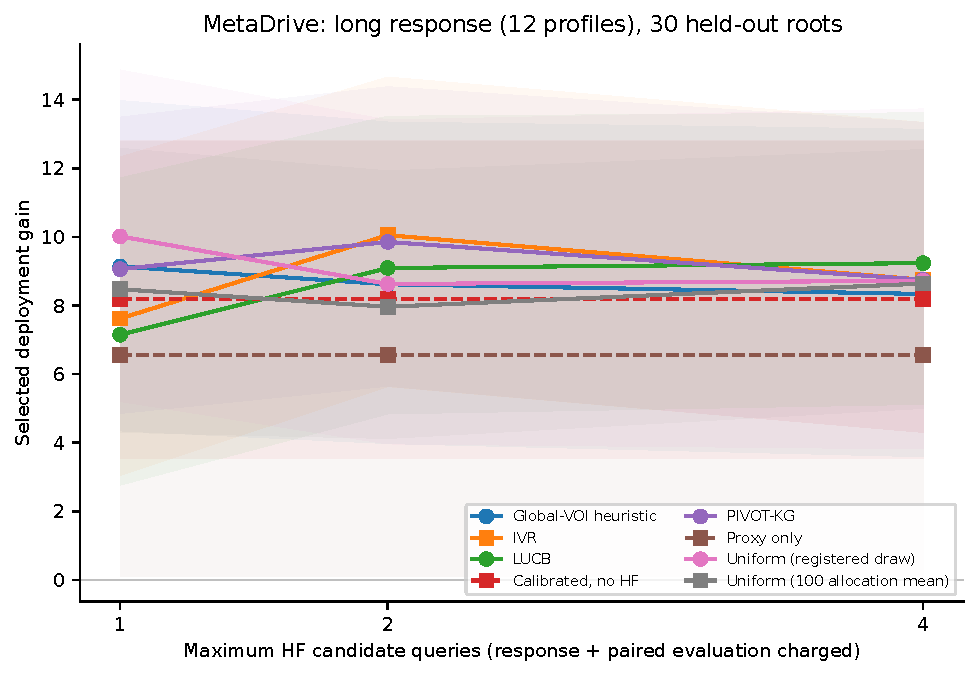
\includegraphics[width=\linewidth]{additions_20260923/metadrive/figures/matched_posterior_selected_audit_gain.pdf}
\caption{First-cohort MetaDrive confirmation: matched-posterior selectors
under the long response condition (12 profiles), 30 independent roots.
Higher independent-audit selected gain is better. The prespecified primary
budget is two candidate queries. Shading gives marginal 95\% root-bootstrap
intervals, not the paired contrast interval; significance must not be inferred
from band overlap. Proxy-only and calibrated no-HF controls cost zero HF
episodes despite being repeated across the query axis.}
\label{add20260923:metadrive:matched_gain}
\end{figure}

\begin{figure}[t]
\centering
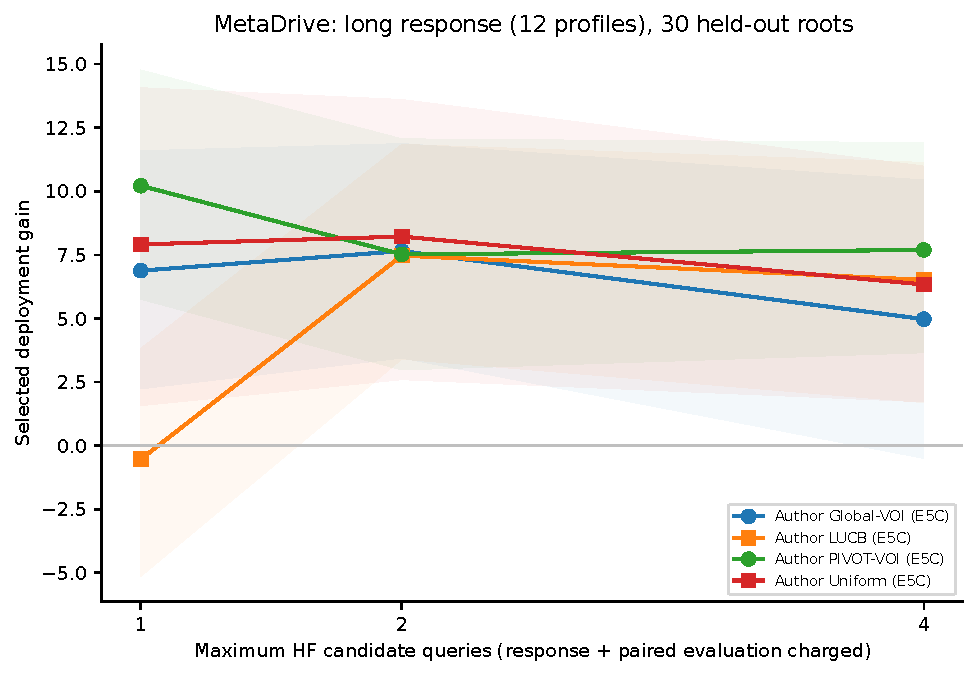
\includegraphics[width=\linewidth]{additions_20260923/metadrive/figures/author_E5C_selected_audit_gain.pdf}
\caption{Separate author E5C implementations on the same first-cohort
MetaDrive confirmation roots and long response condition. These curves are
secondary comparisons. At two queries, the paired PIVOT-VOI minus Uniform
interval includes zero. The shaded marginal intervals have the same
interpretation as in Figure~\ref{add20260923:metadrive:matched_gain}.}
\label{add20260923:metadrive:author_gain}
\end{figure}

\paragraph{Response mechanism: post-hoc diagnostics.}
On the completed 30-root confirmation bank, the long response increases
background return relative to fixed controllers by
$16.811$ [$13.263,20.443$]. The mean absolute discrepancy between fixed-background
and responding-background update gains is 9.392 for short response and
12.188 for long response; their paired difference is
$2.796$ [$0.945,4.844$] (Table~\ref{add20260923:metadrive:mechanism}).
Here the fixed-background reference is measured on matched independent audit
scenarios; it is not a re-labelling of the original four-scenario proxy score.
Twelve candidate/root pairs across nine roots have a positive fixed-background
gain and a negative long-response gain in both independent audit streams;
nine of these pairs also have positive original proxy scores.
These diagnostics support the occurrence of response-induced improvement
mismatch in this setting. They were computed after cohort completion and do
not replace the prespecified primary method test.

\begin{table}[t]
\centering
\small
\caption{Post-hoc mechanism diagnostics on the 30 confirmation roots. ``Short'' and ``long'' search 4 and 12 background-controller profiles, respectively. The gain gap compares an update under fixed and responding backgrounds using matched independent audit scenarios. These diagnostics were computed after the first cohort completed and are not its prespecified primary method test.}
\label{add20260923:metadrive:mechanism}
\begin{tabular}{lrr}
\hline
Quantity & Mean & 95\% CI \\
\hline
Background return: long $-$ fixed & $+16.811$ & $[13.263,20.443]$ \\
Absolute update-gain gap: short & $9.392$ & $[7.819,10.896]$ \\
Absolute update-gain gap: long & $12.188$ & $[10.698,13.699]$ \\
Gap: long $-$ short & $+2.796$ & $[0.945,4.844]$ \\
\hline
\end{tabular}
\end{table}


\paragraph{Interpretation and cohort boundary.}
The first cohort supplies evidence for the motivating mechanism while leaving
the primary method advantage unresolved. It does not show that a larger
response gap necessarily produces larger PIVOT gains, nor that PIVOT is
ineffective in general. Absolute regret against a maximum of noisy audit
means is not used as the primary endpoint because that maximum has selection
bias. This addition contains only the first completed cohort; an independently
seeded precision follow-up is a separate cohort and contributes no result here.
